%%%%%%%%%%%%%%%%%%%%%%%%%%%%%%%%%%%%%%%%%%%%%%%%%%%%%%
% Thanks to Xu Minghao's work                        %
% I modify it into uchicago version                  %
% to not make new bug, I don't alter "Ritsumeikan"   %
% keywords in file. Pls feel free to use             %
%%%%%%%%%%%%%%%%%%%%%%%%%%%%%%%%%%%%%%%%%%%%%%%%%%%%%%

%%%%%%%%%%%%%%%%%%%%%%%%%%%%%%%%%%%%%%%%%%%%%%%%%%%%%%
% A Beamer template for Ritsumeikan University       %
% Author: Ming-Hao Xu (Xu Minghao)                   %
% Date:   April 2022.                                %
% LPPL Licensed.                                     %
%%%%%%%%%%%%%%%%%%%%%%%%%%%%%%%%%%%%%%%%%%%%%%%%%%%%%%

\documentclass[spanish]{beamer}
\usepackage{multicol}
\usepackage{Ritsumeikan}
\usepackage[export]{adjustbox}
\usepackage{hyperref}
\usepackage[T1]{fontenc}
\usepackage[backend=bibtex,style=ieee,maxnames=1,minnames=1]{biblatex}
\addbibresource{ref.bib}
% other packages
\usepackage{latexsym,amsmath,xcolor,multicol,booktabs,calligra}
\usepackage{graphicx,pstricks,listings,stackengine}
\usepackage{tikz}
\usepackage{media9}
\usepackage{multimedia}
\usepackage{caption}
\usepackage{tabularx}
\usepackage{xcolor}
\usepackage{colortbl}
\usepackage{adjustbox}
% dummy text; remove it when working on this template
\usepackage{pifont}
\newcommand{\xmark}{\ding{55}}
\newcommand{\cmark}{\textcolor{green!60!black}{\ding{51}}}%
\newcommand{\qmark}{\textcolor{orange}{\textbf{?}}}%
\usepackage{lipsum}
%Language Packages
\usepackage[spanish]{babel}

\usepackage{ragged2e}
\justifying%

\addto\captionsspanish{\renewcommand{\tablename}{Tabla}}

% Definir nuevos comandos para los integrantes y la facultad
\author[Carrillo B. José E. \&  Robles O. José A.]{Carrillo Barreiro José Emiliano \\ Robles Ortero José Ángel}
\title{Trabajo Terminal No. 2025-B065}
\subtitle{Modelo para representar la interacción gravitacional de dos cuerpos}
\institute{Instituto Politécnico Nacional \\ Escuela Superior de Cómputo}
\newcommand{\directortesis}{Dr.\ Cesar Hernández Vasquez}
\newcommand{\codirectortesis}{Dr.\ Mauricio Olguín Carbajal}
\date{\today}

% defs
\def\cmd#1{\texttt{\color{red}\footnotesize $\backslash$#1}}
\def\env#1{\texttt{\color{blue}\footnotesize #1}}
\definecolor{deepblue}{rgb}{0,0,0.5}
\definecolor{ccnuMainColor}{RGB}{0,86,109}
\definecolor{deepgreen}{rgb}{0,0.5,0}
\definecolor{halfgray}{gray}{0.55}


\lstset{
    basicstyle=\ttfamily\small,
    keywordstyle=\bfseries\color{deepblue},
    emphstyle=\ttfamily\color{ccnuMainColor},    % Custom highlighting style
    stringstyle=\color{deepgreen},
    numbers=left,
    numberstyle=\small\color{halfgray},
    rulesepcolor=\color{red!20!green!20!blue!20},
    frame=shadowbox,
}


\begin{document}

    \begin{frame}
        \titlepage%
    \end{frame}

    \include{secciones/01-introduccion}
    \section{Estado del Arte}

\begin{frame}{Estado del arte}
    \centering
    \captionof{table}{Comparativa contra soluciones disponibles}%
    \label{tab:arte}
    \vspace{-0.1cm}
    \begin{adjustbox}{max width=0.9\textwidth,max height=0.7\textheight, keepaspectratio}
        \renewcommand{\arraystretch}{1.3}
            \begin{tabular}{@{}>{\bfseries}p{0.35\textwidth} p{0.4\textwidth} p{0.20\textwidth} p{0.15\textwidth} p{0.35\textwidth}@{}}
            \toprule
            \textbf{Producto o metodo} & \textbf{Características} & \textbf{Escalabilidad} & \textbf{Usa IA} & \textbf{Cambios dinamicos} \\
            \midrule
            ode\_num\_int & Framework C++11 modular para EDOs; orientado a pruebas de integradores. & Media & No & No \\
            Representación Geométrica & Quadtrees/Octrees para geometría eficiente, no simula dinámica. & Alta & No & No \\
            Método n-NNN & Simulación con n-vecinos y cirugía Hamiltoniana; inspirado en IA. & Alta & Sí & No \\
            PKDGRAV3 & Hidrodinámica sin malla (MFM/MFV); vecinos adaptativos. & Alta & No & No \\
            \bottomrule
            \end{tabular}
    \end{adjustbox}
    \smallskip
\end{frame}



\begin{frame}{Estado del arte}
    \centering
    \captionof{table}{Comparativa contra soluciones disponibles}%
    \label{tab:arte}
    \vspace{-0.1cm}
    \begin{adjustbox}{max width=0.9\textwidth,max height=0.7\textheight, keepaspectratio}
        \renewcommand{\arraystretch}{1.3}
            \begin{tabular}{@{}>{\bfseries}p{0.35\textwidth} p{0.4\textwidth} p{0.20\textwidth} p{0.15\textwidth} p{0.35\textwidth}@{}}
            \toprule
            \textbf{Producto o metodo} & \textbf{Características} & \textbf{Escalabilidad} & \textbf{Usa IA} & \textbf{Cambios dinamicos} \\
            \midrule
            SPH/N-body Híbrido & Interacciones gas-estrella con árbol Barnes-Hut y pasos bloque. & Alta & No & No \\
            Integrador Simpléctico & Orden 2+, reversible; ideal para colisiones. & Media & No & No \\
            Solver TPM & Combina PM y Tree según densidad local; altamente paralelizado. & Alta & No & No \\
            Algoritmo TPM & Descomposición por densidad; integración multi-escala. & Alta & No & No \\
            \bottomrule
            \end{tabular}
    \end{adjustbox}
    \smallskip
\end{frame}


\begin{frame}{Estado del arte}
    \centering
    \captionof{table}{Comparativa contra soluciones disponibles}%
    \label{tab:arte}
    \vspace{-0.1cm}
    \begin{adjustbox}{max width=0.9\textwidth,max height=0.7\textheight, keepaspectratio}
        \renewcommand{\arraystretch}{1.3}
            \begin{tabular}{@{}>{\bfseries}p{0.35\textwidth} p{0.4\textwidth} p{0.20\textwidth} p{0.15\textwidth} p{0.35\textwidth}@{}}
            \toprule
            \textbf{Producto o metodo} & \textbf{Características} & \textbf{Escalabilidad} & \textbf{Usa IA} & \textbf{Cambios dinamicos} \\
            \midrule
            REBOUND & Modular; incluye varios integradores, colisiones y condiciones frontera. & Alta & No & No \\
            Estabilidad Planetaria & Estudio con REBOUND; Gini vs. inestabilidad. No eventos internos. & Alta & No & No \\
            \midrule
            \rowcolor{yellow!20}
            \textbf{Solución Propuesta} & \textbf{Combina FMM/Barnes-Hut para cálculo gravitacional eficiente con Algoritmos Bioinspirados para la \textit{optimización y ajuste dinámico} de parámetros (masa) durante la simulación.}  & \textbf{Alta} & \textbf{SÍ} & \textbf{SÍ} \\
            \bottomrule
            \end{tabular}
    \end{adjustbox}
    \smallskip
\end{frame}

    \section{Marco Teórico}
\subsection[Tecnologías]{Tecnologías: Lenguaje \& Librerias.}

\begin{frame}{Lenguaje de Programación}{Python}
    \begin{columns}
        \begin{column}{0.4\textwidth}
            % Aquí podrías incluir una imagen de ejemplo
            \centering
            \begin{figure}[H]
                \centering
                \adjustbox{max width=\textwidth, max height=0.5\textheight}{%
                
\includegraphics{img/marcoTeorico/python-logo.png}
                }
                \vspace{-0.25cm}
                \caption{\tiny~Logo de Python \textit{Adaptado de:}~\cite{PythonSoftwareFoundation}}%
                \label{fig:Python_logo}
            \end{figure}
        \end{column}
        \begin{column}{0.6\textwidth}
            \begin{itemize}
                \item Alto nivel y propósito general
                \item Sintaxis clara
                \item Multiparadigma
                \item Tipado dinámico
                \item Extensa biblioteca
            \end{itemize}
        \end{column}
    \end{columns}
\end{frame}

\begin{frame}{Biblioteca de Simulación N-Cuerpos}{REBOUND}
    \begin{columns}
        \begin{column}{0.6\textwidth}
            \begin{itemize}
                \item Implementado en C
                \item Dinámica colisional y no colisional
                \item Integradores avanzados
                \item Algoritmos de gravedad
                \item Detección y resolución de colisiones
            \end{itemize}
        \end{column}
        \begin{column}{0.4\textwidth}
            % Aquí podrías incluir una imagen de ejemplo
            \centering
            \begin{figure}[H]
                \centering
                \adjustbox{max width=1.4\textwidth, max height=0.5\textheight}{%
                
\includegraphics{img/marcoTeorico/reboundblack-logo.png}
                }
                \vspace{-0.25cm}
                \caption{\tiny~Logo de REBOUND \textit{Adaptado de:}~\cite{Rein2012}}%
                \label{fig:REBOUND_logo}
            \end{figure}
        \end{column}
    \end{columns}
\end{frame}

\begin{frame}{Biblioteca de Optimización}{pymoo}
    \begin{columns}
        \begin{column}{0.4\textwidth}
            % Aquí podrías incluir una imagen de ejemplo
            \centering
            \begin{figure}[H]
                \centering
                \adjustbox{max width=\textwidth, max height=0.5\textheight}{%
                
\includegraphics{img/marcoTeorico/pymoo-logo.png}
                }
                \vspace{-0.25cm}
                \caption{\tiny~Logo de pymoo \textit{Adaptado de:}~\cite{blank2020}}%
                \label{fig:pymoo_logo}
            \end{figure}
        \end{column}
        \begin{column}{0.6\textwidth}
            \begin{itemize}
                \small
                \item Framework para optimización
                \item Amplia gama de algoritmos
                \item Alta flexibilidad
                \item Uso de herramientas específicas
                \item Soporte para paralelización
            \end{itemize}
        \end{column}
    \end{columns}
\end{frame}

\begin{frame}{Biblioteca de Visualización}{Matplotlib}
    \begin{columns}
        \begin{column}{0.6\textwidth}
            \begin{itemize}
                \item Biblioteca de visualización
                \item Gran flexibilidad y personalización
                \item Gráficos científicos
                \item Amplia documentación
            \end{itemize}
        \end{column}
        \begin{column}{0.4\textwidth}
            % Aquí podrías incluir una imagen de ejemplo
            \centering
            \begin{figure}[H]
                \centering
                \adjustbox{max width=\textwidth, max height=0.5\textheight}{%
                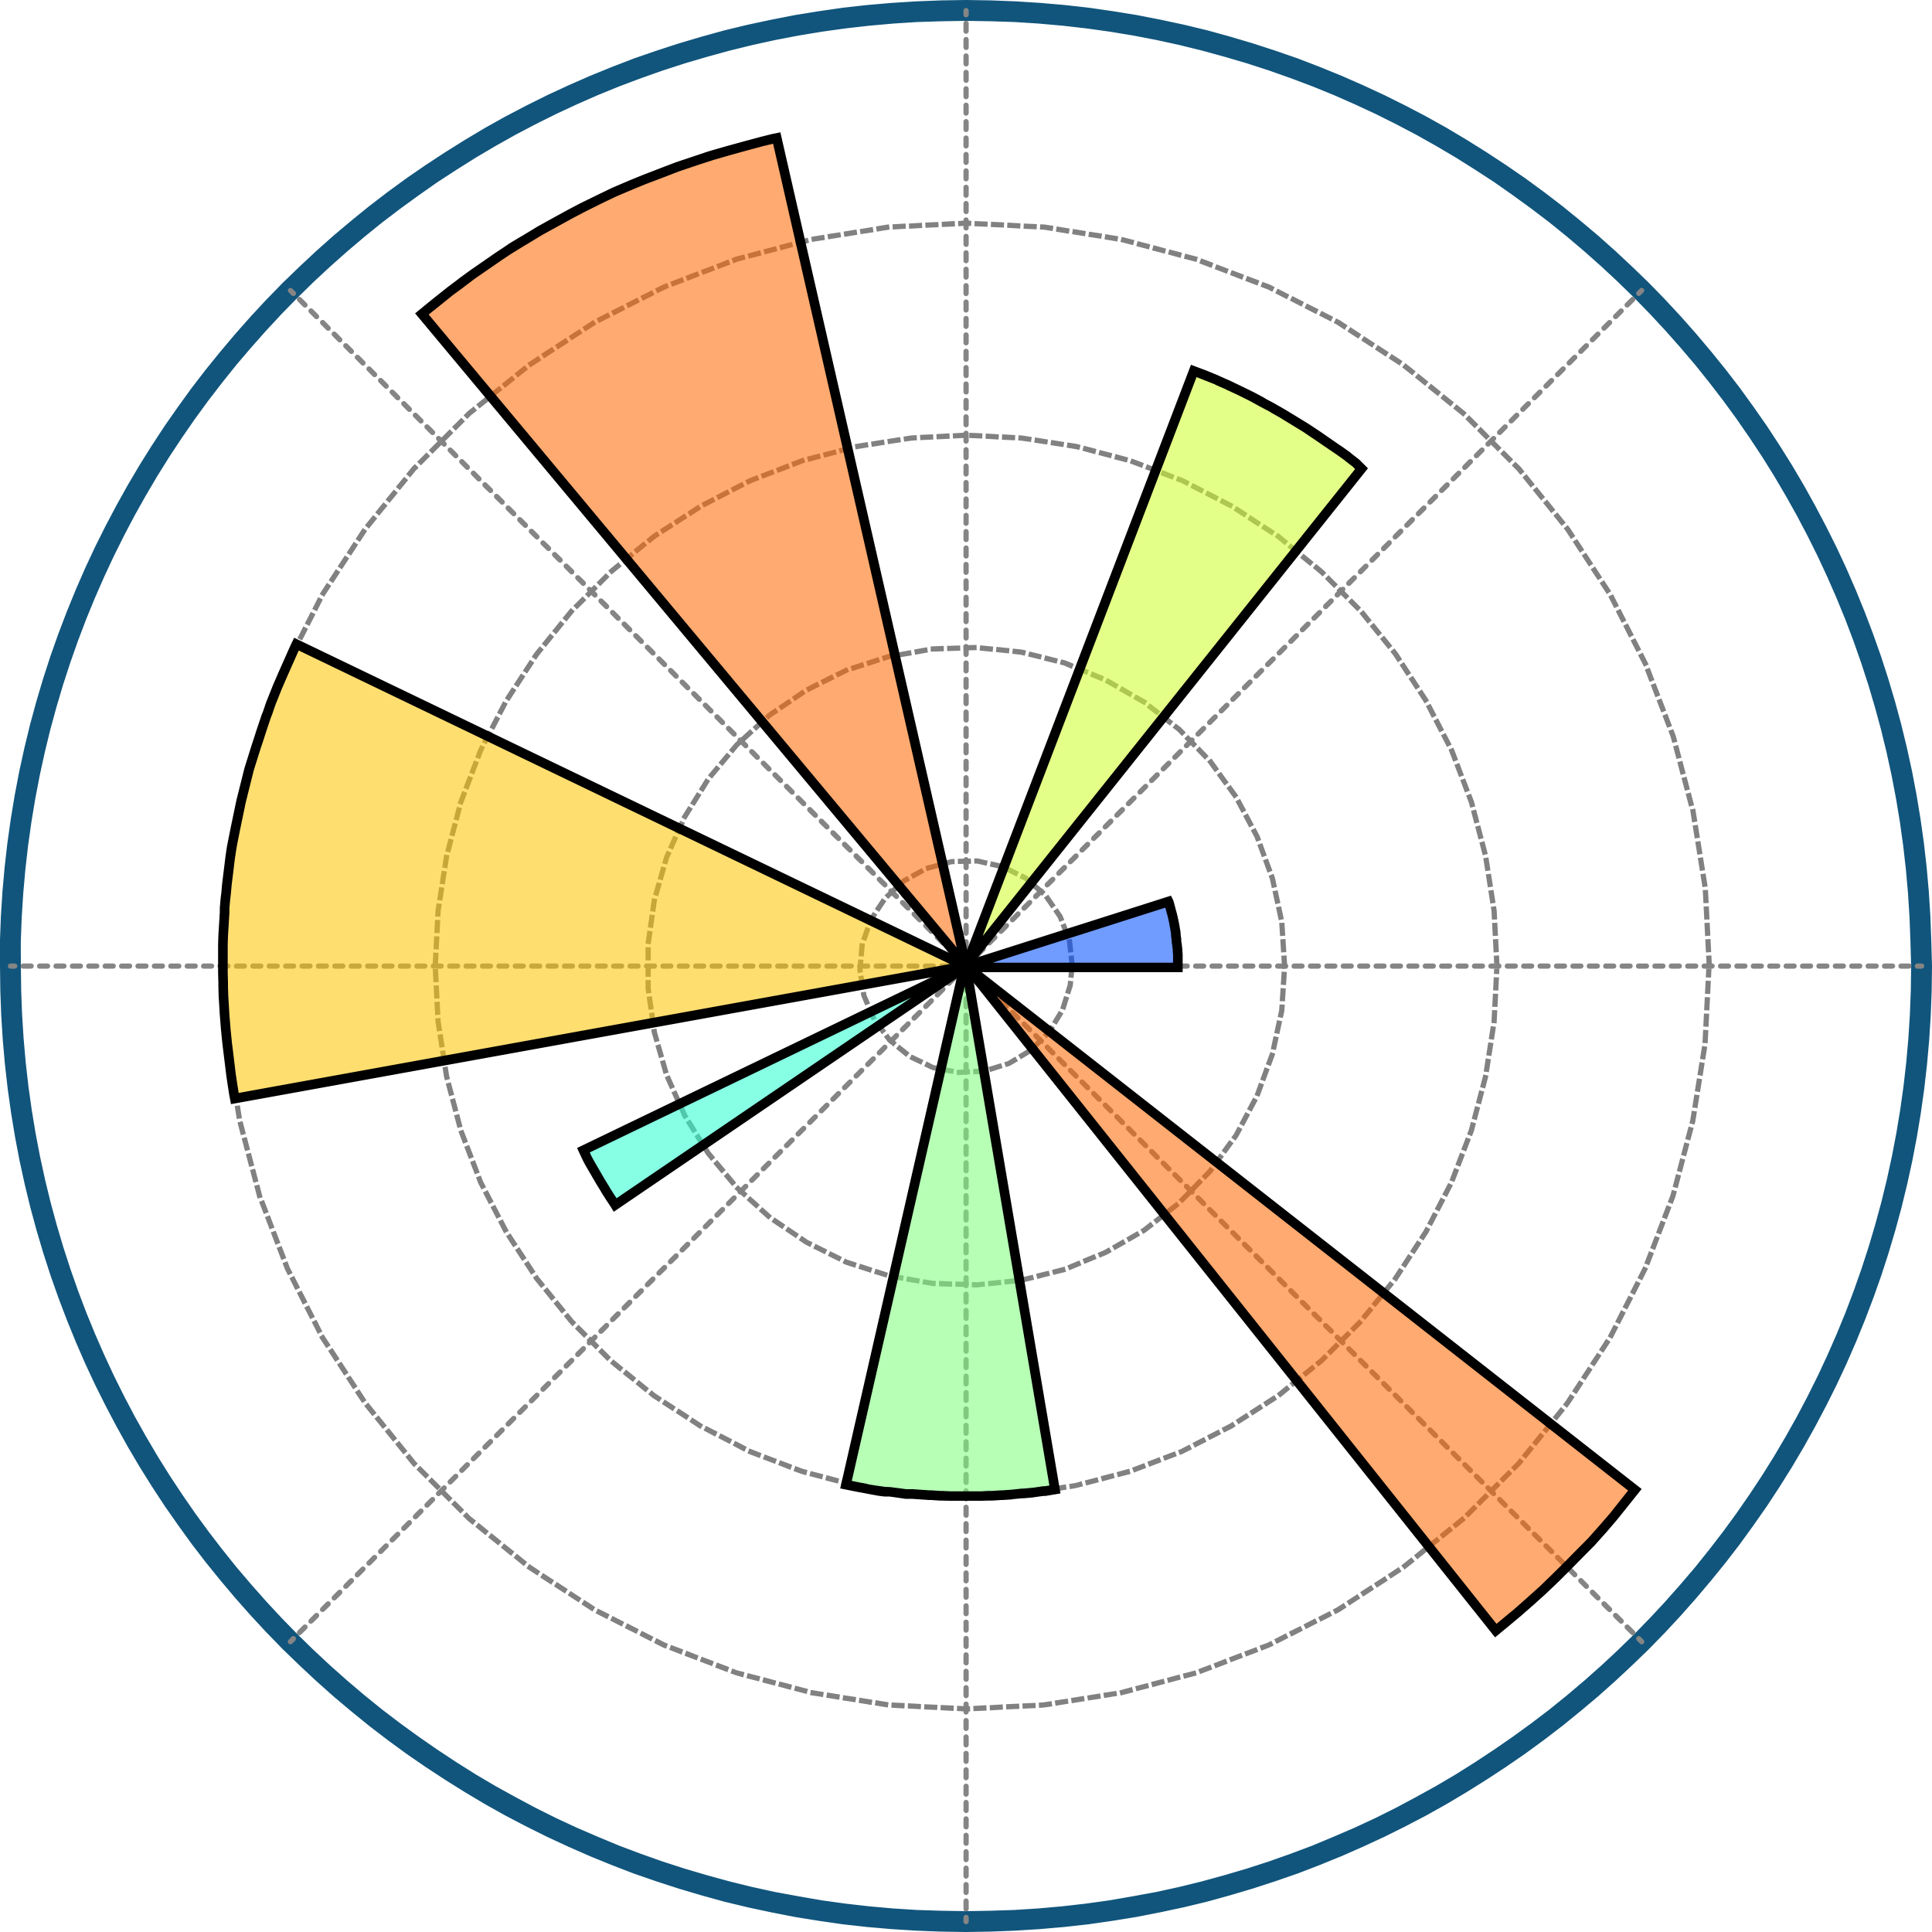
\includegraphics{img/marcoTeorico/matplotlib-logo.png}
                }
                \vspace{-0.25cm}
                \caption{\tiny~Logo de Matplotlib \textit{Adaptado de:}~\cite{Hunter:2007}}%
                \label{fig:Matplotlib_logo}
            \end{figure}
        \end{column}
    \end{columns}
\end{frame}

\begin{frame}{Biblioteca de GUI para Python}{PyQt}
    \begin{columns}
        \begin{column}{0.4\textwidth}
            % Aquí podrías incluir una imagen de ejemplo
            \centering
            \begin{figure}[H]
                \centering
                \adjustbox{max width=\textwidth, max height=0.5\textheight}{%
                
\includegraphics{img/marcoTeorico/qt-logo.png}
                }
                \vspace{-0.25cm}
                \caption{\tiny~Logo de PyQt.~\textit{Adaptado de:}~\cite{qt_wiki}}%
                \label{fig:PyQt_logo}
            \end{figure}
        \end{column}
        \begin{column}{0.6\textwidth}
            \begin{itemize}
                \item Basado en Qt (C++)
                \item Widgets y \textit{layouts}
                \item Integración con Matplotlib
                \item Soporte para multihilo
                \item Qt Designer
            \end{itemize}
        \end{column}
    \end{columns}
\end{frame}

\subsection[Métodos \& Técnicas]{Métodos \& Técnicas a utilizar.}

\begin{frame}{Cálculo de Gravedad y Colisiones}{Mediante módulos de \texttt{REBOUND}}
    \begin{columns}
        \begin{column}{0.6\textwidth}
            \small
            \begin{itemize}
                \item \textbf{Cálculo de Gravedad:}
                \begin{itemize}
                    \item \textbf{Suma Directa:} $O(N \cdot N_{\text{active}})$
                    \item \textbf{Octree (Barnes-Hut):} $O(N \log N)$
                \end{itemize}
                \item \textbf{Detección de Colisiones:}
                \begin{itemize}
                    \item \textbf{Búsqueda Directa:} $O(N^2)$
                    \item \textbf{Octree:} $O(N \log N)$
                    \item \textbf{Barrido Plano}
                \end{itemize}
            \end{itemize}
        \end{column}
        \begin{column}{0.4\textwidth}
            % Aquí podrías incluir una imagen de ejemplo
            \centering
            \begin{figure}[H]
                \centering
                \adjustbox{max width=\textwidth, max height=0.5\textheight}{%
                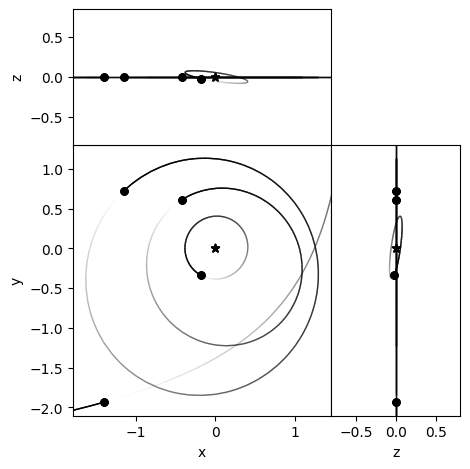
\includegraphics{img/marcoTeorico/rebound-simulation.png}
                }
                \vspace{-0.25cm}
                \caption{\tiny~Simulación de orbitas usando REBOUND \textit{Adaptado de:}~\cite{rebound_hyperbolic_orbits_2025}}%
                \label{fig:REBOUND_methods}
            \end{figure}
        \end{column}
    \end{columns}
\end{frame}

\begin{frame}{Algoritmo de Exploración}{Algoritmo Genético (AG) con pymoo}
    \begin{columns}
        \begin{column}{0.6\textwidth}
            \small
            \begin{itemize}
                \item \textbf{Componentes principales:}
                \begin{itemize}
                    \item \textbf{Muestreo}
                    \item \textbf{Selección de Padres}
                    \item \textbf{Cruce}
                    \item \textbf{Mutación}
                    \item \textbf{Manejo de Restricciones}
                \end{itemize}
            \end{itemize}
        \end{column}
        \begin{column}{0.4\textwidth}
            % Aquí podrías incluir una imagen de ejemplo
            \centering
            \begin{figure}[H]
                \centering
                \adjustbox{max width=\textwidth, max height=0.5\textheight}{%
                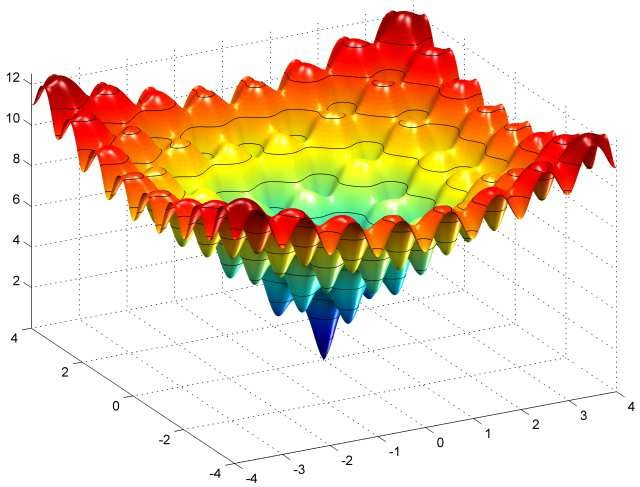
\includegraphics{img/marcoTeorico/benchmarkfunction.png}
                }
                \vspace{-0.25cm}
                \caption{\tiny~Funcion tipo benchmark, para la evaluación de AGs \textit{Adaptado de:}~\cite{silva2018}}%
                \label{fig:genetic_algorithm}
            \end{figure}
        \end{column}
    \end{columns}
\end{frame}

\begin{frame}{Indicador de Estabilidad}{Exponente de Lyapunov}
    \begin{columns}
        \begin{column}{0.4\textwidth}
            % Aquí podrías incluir una imagen de ejemplo
            \centering
            \begin{figure}[H]
                \centering
                \adjustbox{max width=\textwidth, max height=0.5\textheight}{%
                
\includegraphics{img/marcoTeorico/lyapunovExponent-in-randomAttractors.jpg}
                }
                \vspace{-0.25cm}
                \caption{\tiny~Atractor caótico generado mediante exponentes de Lyapunov.~\textit{Adaptado de:}~\cite{bourke_lyapunov_attractors_2001}}%
                \label{fig:Lyapunov_diagram}
            \end{figure}
        \end{column}
        \begin{column}{0.6\textwidth}
            \begin{itemize}
                \item Cuantifica sensibilidad
                \item Indicador primario de estabilidad/caos
                \item Medida objetiva y cuantitativa
                \item Predice comportamiento a largo plazo
                \item Base matemática rigurosa
            \end{itemize}
        \end{column}
    \end{columns}
\end{frame}

\begin{frame}{Enfoque del Proyecto}{Factibilidad y Optimización}
    \begin{columns}
        \begin{column}{0.4\textwidth}
            % Aquí podrías incluir una imagen de ejemplo
            \centering
            \begin{figure}[H]
                \centering
                \adjustbox{max width=\textwidth, max height=0.5\textheight}{%
                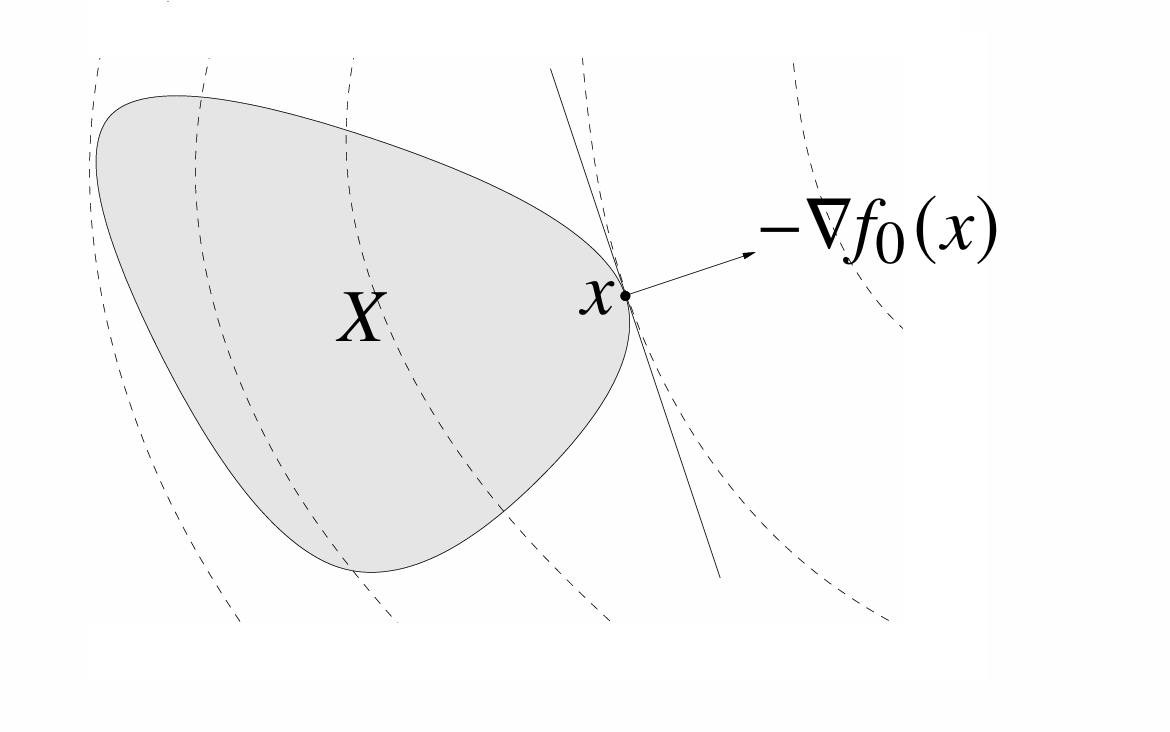
\includegraphics{img/marcoTeorico/optimizacion_fig1.png}
                }
                \vspace{-0.25cm}
                \caption{\tiny~Gráfica 2D que muestre contornos de una función objetivo $f_0(x)$,
                        una región factible sombreada definida por restricciones, y el punto óptimo $x^*$.\ \textit{Adaptado de:}~\cite{BoydVandenbergheSlides2023}}%
                \label{fig:factibility_optimization}
            \end{figure}
        \end{column}
        \begin{column}{0.6\textwidth}
            \small
            \begin{itemize}
                \item \textbf{Problema de Factibilidad:}
                \begin{itemize}
                    \item Determinar si existen configuraciones estables
                    \item Criterio clave: Exponente de Lyapunov $\lambda_1 \leq \text{umbral}$
                    \item Restricciones físicas. %masas positivas, parámetros orbitales válidos
                \end{itemize}
                \item \textbf{Marco de Optimización:} % (Herramienta)
                \begin{itemize}
                    \item Función objetivo: minimizar $\lambda_1$ directamente
                    \item Algoritmo Genético como herramienta exploratoria
                    \item Permite búsqueda eficiente en el espacio de parámetros
                \end{itemize}
            \end{itemize}
        \end{column}
    \end{columns}
\end{frame}
    \section{Planeación}
    \section{Análisis}

\begin{frame}{Matríz de procesos}
    \centering
    \captionof{table}{Matríz de procesos}
    \label{tab:procesos}
    \vspace{-0.1cm}
    \begin{adjustbox}{max width=0.9\textwidth,max height=0.7\textheight, keepaspectratio}
        \renewcommand{\arraystretch}{1.3}
            \begin{tabular}{@{}>{\bfseries}p{0.35\textwidth}  p{0.35\textwidth} p{0.35\textwidth}@{}}
            \toprule
            \textbf{Nombre del proceso} & \textbf{Objetivo} & \textbf{Salidas}  \\
            \midrule
            \textbf{Captura Parámetros} & Recopilar, validar y almacenar parámetros de configuración del usuario. & Estructura \texttt{\seqsplit{ConfigurationData}} validada, estado de UI actualizado. \\
            \midrule
            \textbf{Mostrar Resultados} & Presentar solución óptima y visualización final al usuario. & Actualización visual de la UI con resultados finales. \\
            \midrule
            \textbf{Evaluar Fitness} & Calcular fitness penalizado (\texttt{\seqsplit{F}\_p}) combinando LE y violaciones. & Valor numérico de $F_p(x)$. \\
            \midrule
            \textbf{Crear Nueva Simulación} & Instanciar un nuevo entorno de simulación vacío en \texttt{\seqsplit{REBOUND}}. & Referencia a nuevo objeto \texttt{\seqsplit{Simulation}}. \\
            \bottomrule
            \end{tabular}
    \end{adjustbox}
    \smallskip
\end{frame}


\begin{frame}{Matríz de procesos}
    \centering
    \captionof{table}{Matríz de procesos}
    \label{tab:procesos}
    \vspace{-0.1cm}
    \begin{adjustbox}{max width=0.9\textwidth,max height=0.7\textheight, keepaspectratio}
        \renewcommand{\arraystretch}{1.3}
            \begin{tabular}{@{}>{\bfseries}p{0.35\textwidth}  p{0.35\textwidth} p{0.35\textwidth}@{}}
            \toprule
            \textbf{Nombre del proceso} & \textbf{Objetivo} & \textbf{Salidas}  \\
            \midrule
            \textbf{Agregar Cuerpos} & Añadir una partícula con propiedades físicas a la simulación. & Instancia \texttt{\seqsplit{sim}} modificada con nueva partícula. \\
            \midrule
            \textbf{Iniciar/Ejecutar Simulación} & Ejecutar la integración numérica paso a paso hasta $T_{\max}$. & Estructura \texttt{\seqsplit{SimulationResult}} con trayectoria completa. \\
            \midrule
            \textbf{Recolectar Datos} & Extraer estado actual del sistema en instantes de visualización. & Estructura \texttt{\seqsplit{VisualizationState}} con instantánea del sistema. \\
            \midrule
            \textbf{Generar Gráficos} & Dibujar o actualizar la representación visual en la pantalla. & Representación gráfica actualizada en la UI. \\
            \bottomrule
            \end{tabular}
    \end{adjustbox}
    \smallskip
\end{frame}

\begin{frame}{Diccionario de Datos: Cuerpo celeste}
  \centering
  \captionof{table}{Cuerpo celeste.}
  \label{tab:diccionario_cuerpos_slide}
  \begin{adjustbox}{max width=0.9\textwidth}
    \begin{tabular}{@{}p{3cm} p{4cm} p{1.5cm} p{1.5cm} p{2.5cm}@{}}
      \toprule
      \textbf{Nombre del atributo} & \textbf{Descripción} & \textbf{Tipo} & \textbf{Rango} & \textbf{Ejemplo} \\
      \midrule
      \textbf{masa} & Masa del cuerpo celeste... & \texttt{float} & \(>0\) (positivos)... & 1.0 \\
      \midrule
      \textbf{a} & Semieje mayor de la órbita... & \texttt{float} & \(>0\) (positivos) & 1.0 \\
      \midrule
      \textbf{e} & Excentricidad orbital... & \texttt{float} & [0, 1) & 0.1 \\
      \midrule
      \textbf{inc\_deg} & Inclinación orbital... & \texttt{float} & [0°, 180°] & 30.0 \\
      \midrule
      \textbf{perturba} & Indica si se aplica... & \texttt{bool} & \texttt{True} o \texttt{False} & True \\
      \bottomrule
    \end{tabular}
  \end{adjustbox}
\end{frame}

\begin{frame}{Diccionario de Datos: Simulación}
  \centering
  \captionof{table}{Simulación.}
  \label{tab:diccionario_simulación_slide}
  \begin{adjustbox}{max width=0.9\textwidth}
    \begin{tabular}{@{}p{3cm} p{4cm} p{1.5cm} p{1.5cm} p{2.5cm}@{}}
      \toprule
      \textbf{Nombre del atributo} & \textbf{Descripción} & \textbf{Tipo} & \textbf{Rango} & \textbf{Ejemplo} \\
      \midrule
      \textbf{t\_max} & Tiempo total de simulación... & \texttt{float} & \( > 0 \) (positivos) & 100.0 \\
      \midrule
      \textbf{N\_steps} & Número de pasos a almacenar... & \texttt{entero} & \(>0\) (positivos) & 1000 \\
      \midrule
      \textbf{sim.units} & Unidades de la simulación... & \texttt{texto} & \texttt{AU, yr, Msun} & AU, yr, Msun \\
      \midrule
      \textbf{sim.integrator} & Indica el integrador numérico... & \texttt{texto} & \texttt{ias15, whfast, BS, mercurius} & ias15 \\
      \midrule
      \textbf{x, y, z} & Guarda las posiciones... & \texttt{array(float)} & \(>0\) (positivos) & [5.0, 230.0, 20.0] \\
      \bottomrule
    \end{tabular}
  \end{adjustbox}
\end{frame}

\begin{frame}{Diccionario de Datos: Métricas}
  \centering
  \captionof{table}{Métricas.}
  \label{tab:diccionario_métricas_slide}
  \begin{adjustbox}{max width=0.9\textwidth}
    \begin{tabular}{@{}p{3cm} p{4cm} p{2.5cm} p{1.5cm} p{2.5cm}@{}}
      \toprule
      \textbf{Nombre del atributo} & \textbf{Descripción} & \textbf{Tipo} & \textbf{Rango} & \textbf{Ejemplo} \\
      \midrule
      \textbf{times} & Array que guarda los tiempos... & \texttt{array(float)} & \(>0\) (positivos) & [0.0, 100.0, 200.0] \\
      \midrule
      \textbf{energy} & Energía total del sistema... & \texttt{float} & Valor real & -0.5 \\
      \midrule
      \textbf{a\_arr, a\_pert} & Array que guarda el semieje... & \texttt{array(float)} & \(>0\) (positivos) & [1.0, 1.5, 2.0] \\
      \midrule
      \textbf{e\_arr, e\_pert} & Array que guarda la excentricidad... & \texttt{array(float)} & [0, 1) & [0.1, 0.2, 0.3] \\
      \midrule
      \textbf{Exponente de Lyapunov ($\mathbf{\lambda}$)}& Indica la tasa de crecimiento... & \texttt{float} & Valor real & 0.01 \\
      \bottomrule
    \end{tabular}
  \end{adjustbox}
\end{frame}
    \section{Diseño}
    \section[Conclusiones]{Conclusiones y Trabajo a Futuro}
\begin{frame}{Conclusión}
    \begin{columns}
        \begin{column}{0.6\textwidth}
            \textbf{Durante la primera fase del Trabajo Terminal, se logró:}
            \begin{itemize}
                \item Establecer el planteamiento y la metodología que guiarán el desarrollo de la solución propuesta.
                \item Identificar diversos métodos y técnicas para abordar eficazmente la problemática planteada.
                \item Consultar a expertos para validar el enfoque y alinearlos con los objetivos del proyecto.
            \end{itemize}
        \end{column}
        \begin{column}{0.4\textwidth}
            % Aquí podrías incluir una imagen de ejemplo
            \centering
            \begin{figure}[H]
                \centering
                \adjustbox{max width=\textwidth, max height=0.5\textheight}{%
                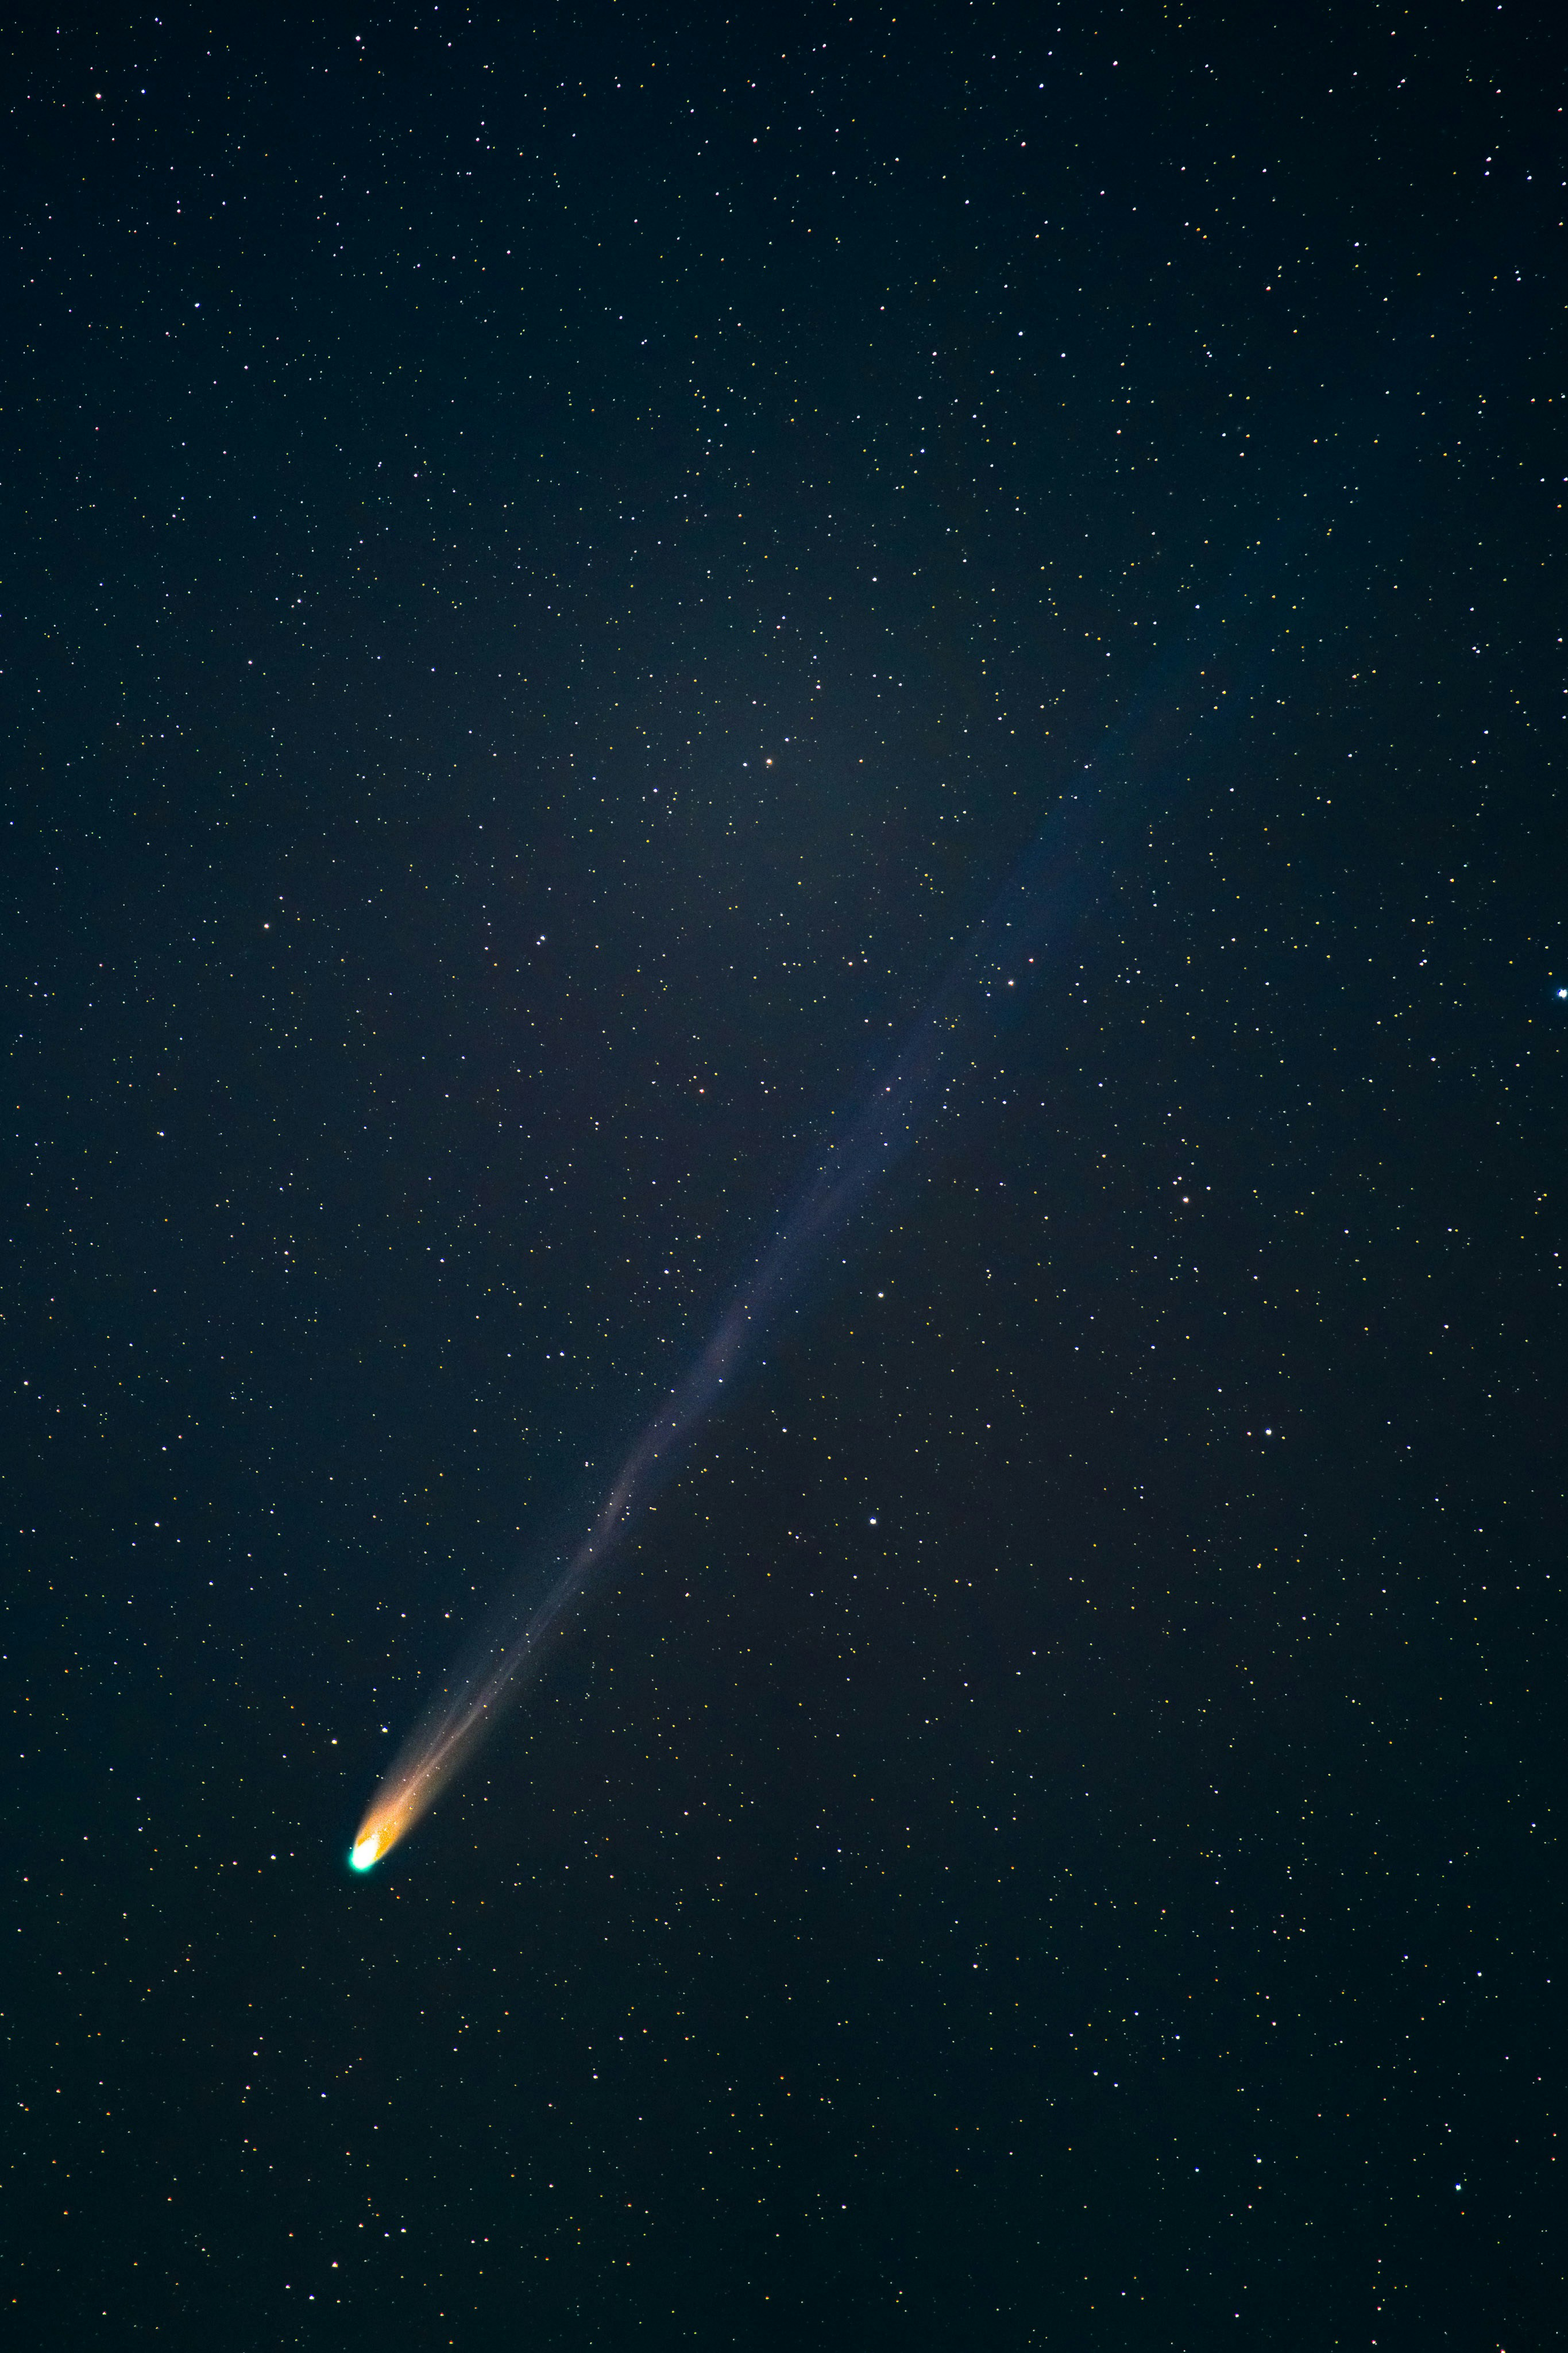
\includegraphics{img/conclusion/cometa.jpg}
                }
                \vspace{-0.25cm}
                \caption{\tiny~Una vista del cielo mirando hacia arriba por la noche \textit{Autoría de:}~\cite{dyer_cielo_nocturno_2021}}%
                \label{fig:Matplotlib_logo}
            \end{figure}
        \end{column}
    \end{columns}
\end{frame}

\begin{frame}{Trabajo a futuro}
    \begin{columns}
        \begin{column}{0.4\textwidth}
            % Aquí podrías incluir una imagen de ejemplo
            \centering
            \begin{figure}[H]
                \centering
                \adjustbox{max width=\textwidth, max height=0.5\textheight}{%
                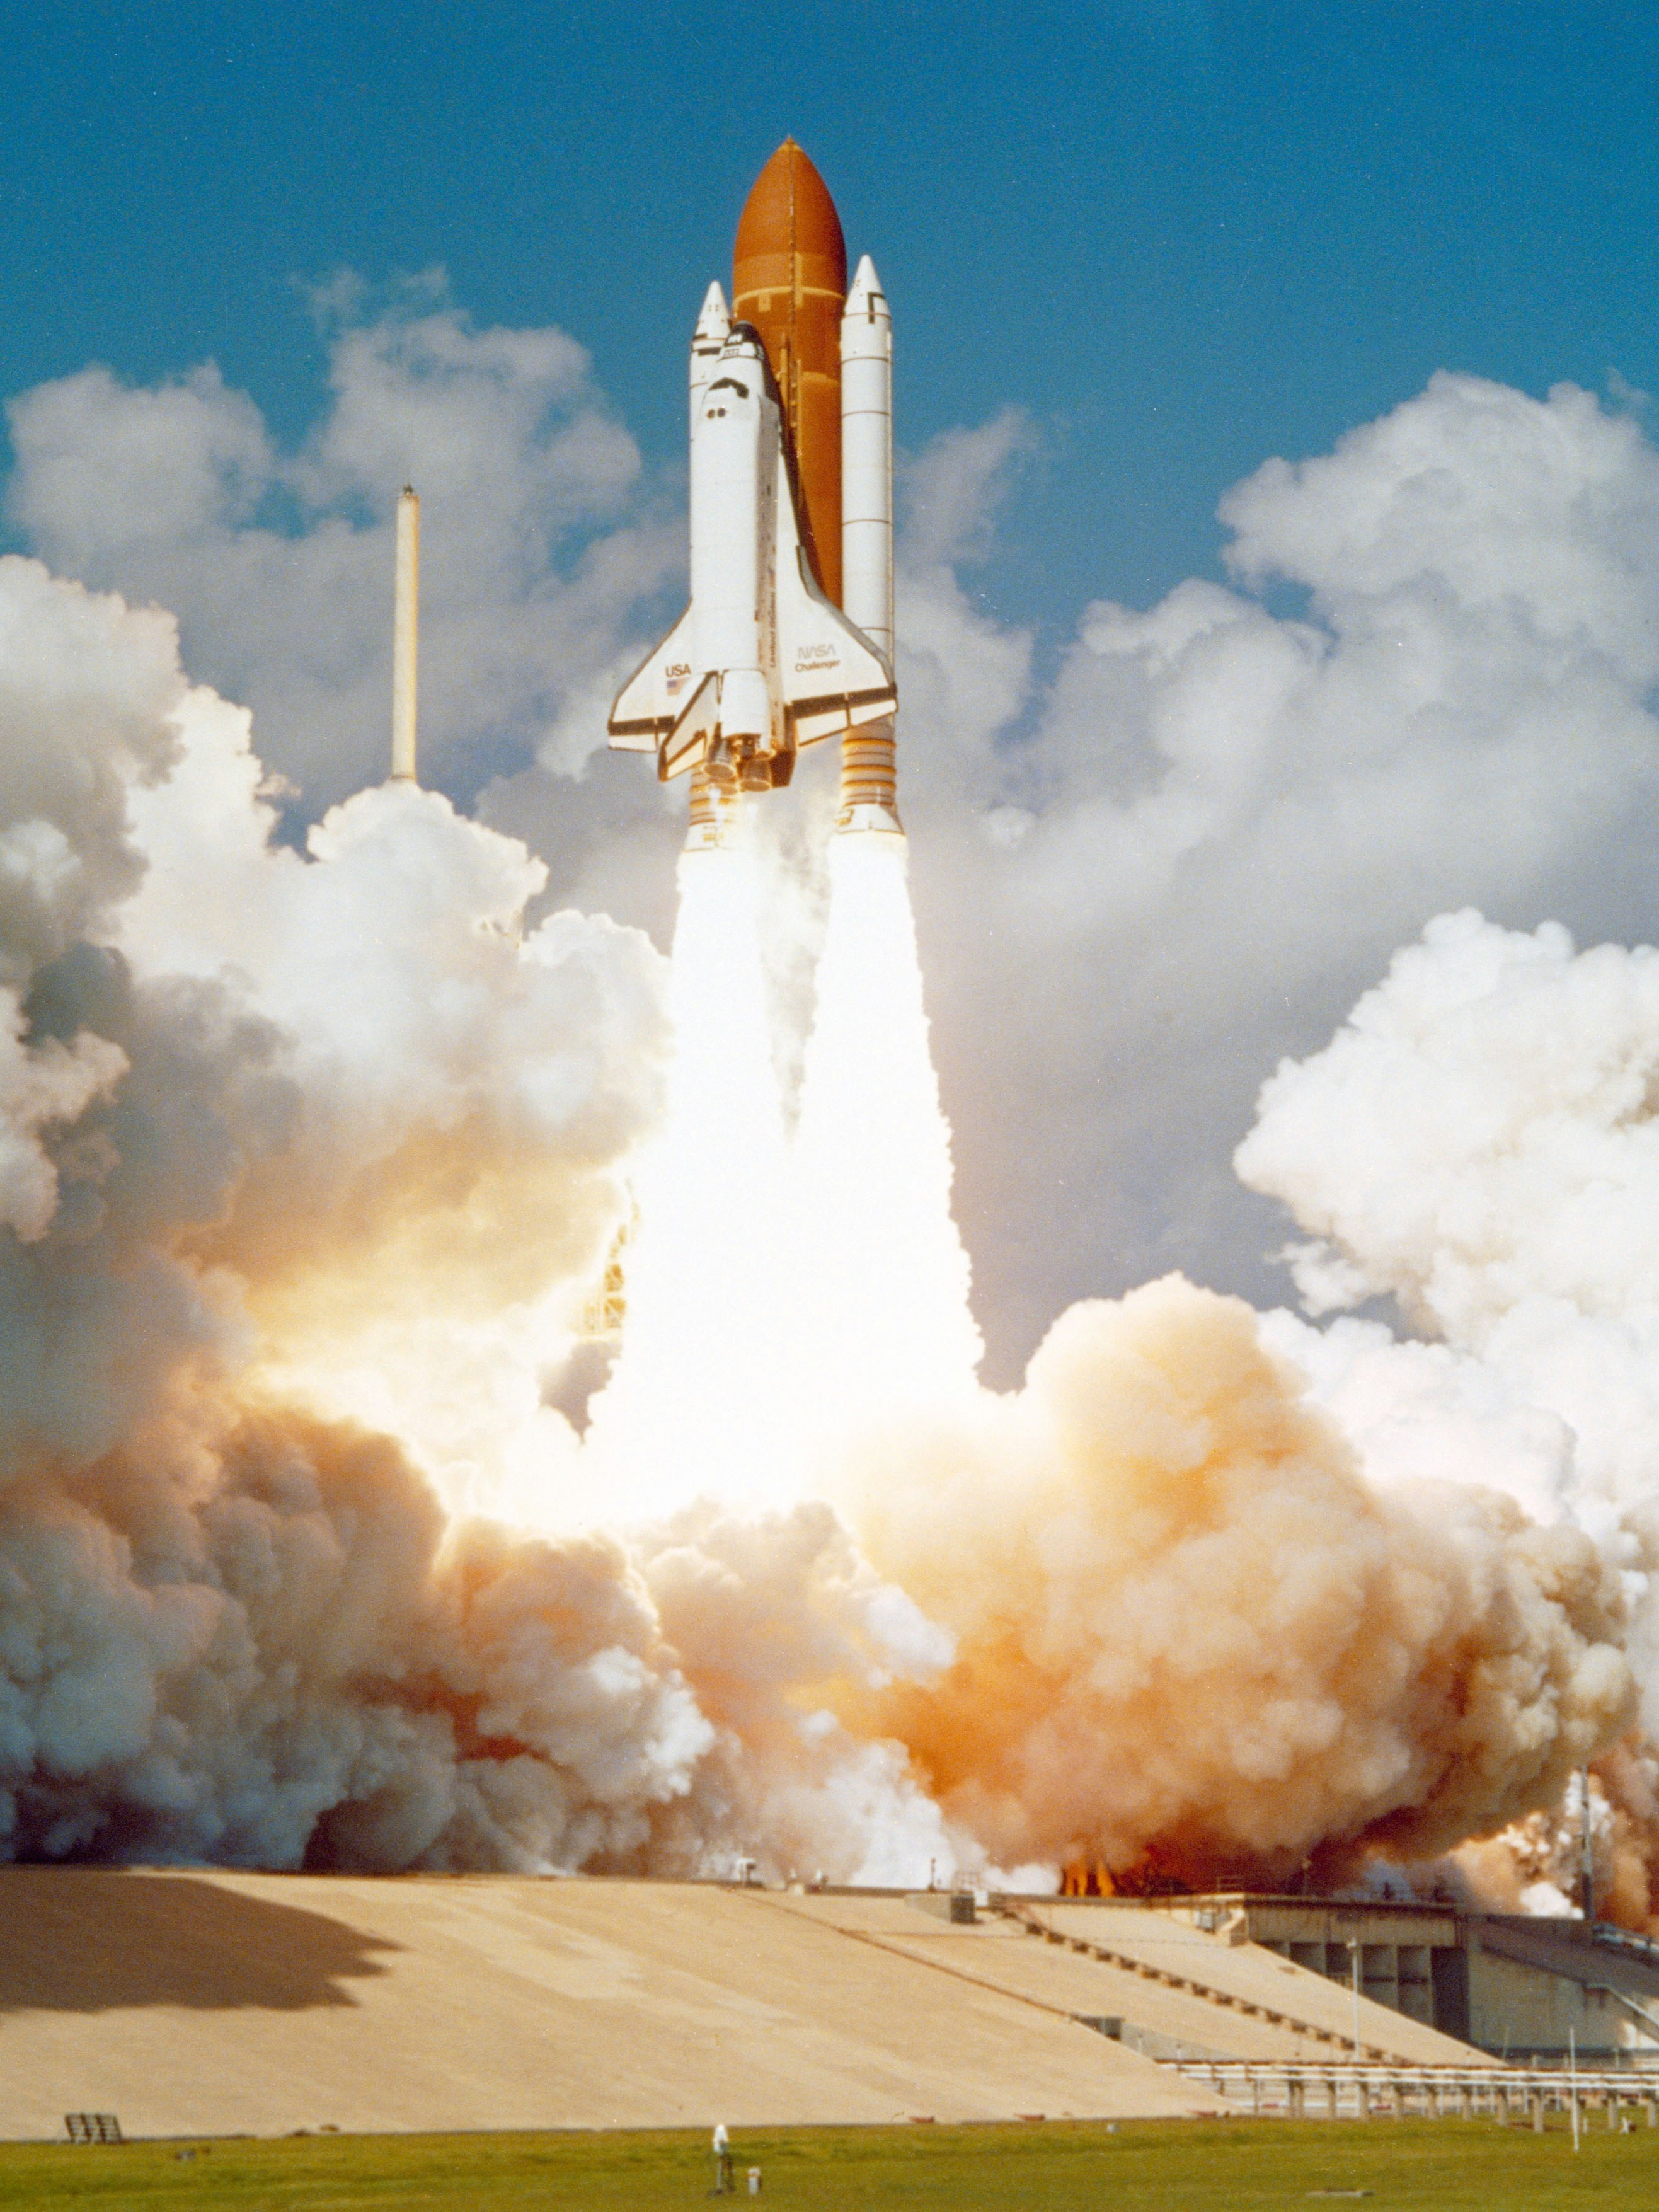
\includegraphics{img/conclusion/spaceshipNasa.jpg}
                }
                \vspace{-0.25cm}
                \caption{\tiny~Transbordador espacial Challenger se lanza desde el Centro Espacial Kennedy.~\textit{Autoría de:}~\cite{nasa_challenger_unsplash}}%
                \label{fig:PyQt_logo}
            \end{figure}
        \end{column}
        \begin{column}{0.6\textwidth}
            Para la siguiente fase del proyecto terminal, se realizarán las siguientes tareas:
            \begin{itemize}
                \item Desarrollo de pseudocódigos
                \item Implementación de módulos.
                \item Pruebas y refinamiento.
                \item Consulta con expertos y miembros del comité sinodal sobre los avances.
                \item Elaboración de un manual de usuario.
            \end{itemize}
        \end{column}
    \end{columns}
\end{frame}

    \section{Referencias}

    \begin{frame}[allowframebreaks]
        \frametitle{Referencias}
        \begingroup
        \fontsize{6pt}{7pt}\selectfont
        \printbibliography[heading=none]
        \endgroup
    \end{frame}

    \begin{frame}
        \begin{center}
            {\Huge\calligra~¡Gracias por su atención!}\\
            ¿Alguna pregunta o comentario?
        \end{center}
    \end{frame}

    \appendix
    \makeatletter
    \renewcommand{\thesection}{\Alph{section}}
    \@addtoreset{section}{part}
    \makeatother
    \setcounter{section}{0}

    \begin{frame}
        \begingroup
            \begin{center}
                {\Huge Anexos}
            \end{center}
        \endgroup
    \end{frame}
    \section{Tablas Comparativas del Marco Teórico}

\begin{frame}{Anexo \thesection~: Lenguaje de Programación}
    \centering
    \captionof{table}{Comparativa de Lenguaje de Programación}%
    \label{tab:comparativa}
    \vspace{-0.1cm}
    \begin{adjustbox}{max width=0.9\textwidth,max height=0.7\textheight, keepaspectratio}
        \renewcommand{\arraystretch}{1.3}
            \begin{tabular}{@{}>{\bfseries}p{0.5\textwidth} p{0.6\textwidth} >{\columncolor{yellow!30}}p{0.6\textwidth}@{}}
            \toprule
            \textbf{Característica} & \textbf{C++} & \textbf{Python} \\
            \midrule
            Velocidad de Ejecución & Máxima. Ideal para cálculos intensivos. & Menor. \\
            Velocidad de Desarrollo & Lento y verboso. & Rápido, claro y flexible para iterar. \\
            Bibliotecas Científicas & Potentes, pero más complejas de integrar. & Vastas y accesibles. \\
            Visualización & Requiere herramientas externas. & Fácil con Matplotlib, Plotly o Bokeh. \\
            Integración con REBOUND & Directa con linking C. & Interfaz oficial en Python lista para usar. \\
            Algoritmos Bioinspirados & Óptimo si se implementan desde cero. & Fáciles de coordinar o conectar con código externo. \\
            Gestión de Memoria & Manual. Mayor control. & Automática. Simplifica el desarrollo. \\
            Curva de Aprendizaje & Alta.. & Baja a moderada.. \\
            Prototipado / Experimentación & Lento. & Ágil. \\
            Depuración & Complejo. & Sencillo. \\
            Enfoque del Proyecto & Control total, pero puede complicar. & Permite centrarse en la solución y resultados. \\
            \bottomrule
            \end{tabular}
    \end{adjustbox}
    \smallskip
\end{frame}


\begin{frame}{Anexo \thesection~: Comparativa de Bibliotecas N-Cuerpos}
    \centering
    \captionof{table}{Comparativa extensa de bibliotecas para simulación N-cuerpos.}%
    \label{tab:nbody-comparativa-beamer}
    \vspace{-0.1cm} % Espacio como en el ejemplo
    \begin{adjustbox}{max width=\textwidth, max height=0.7\textheight, keepaspectratio} % Aumentamos max height
        % Ajustes de la tabla original
        \renewcommand{\arraystretch}{1.2} % Reducido un poco por si acaso, puedes probar 1.3
        \scriptsize % o \tiny si es necesario más pequeño
        %\rowcolors{2}{gray!10}{white} % Colores de fila alternos, empezando por la segunda fila de datos
        \begin{tabular}{
            @{}>{\bfseries}p{0.4\textwidth}
            >{\columncolor{yellow!30}}p{0.3\textwidth}
            p{0.3\textwidth}
            p{0.3\textwidth}
            p{0.3\textwidth}
            p{0.3\textwidth}@{}}
        \toprule
        \textbf{Característica} & \textbf{REBOUND} & \textbf{PKDGRAV3} & \textbf{AMUSE} & \textbf{NBody (Python)} & \textbf{PyGaia} \\
        \midrule

        Lenguaje Principal / Interfaz & C (Python API) & C++ & Python & Python & Python \\

        Enfoque Principal & Colisional/no colisional, sistemas N-cuerpos & Cosmología a gran escala & Framework multipropósito & Simulaciones educativas & Análisis Gaia \\

        Tipos de Problemas & Planetas, cúmulos, anillos & Galaxias, materia oscura & Multifísica astrofísica & Sistemas pequeños & Dinámica galáctica \\

        Algoritmos de Gravedad & Barnes-Hut/Suma directa & TreePM & Hermite/Tree/SPH & Suma directa & Potenciales analíticos \\

        Manejo de Colisiones & Sí (esferas duras) & No & Depende del backend & No & N/A \\

        Integradores Numéricos & WHFast/ IAS15/ Leapfrog & Leapfrog KDK & Hermite/ Symplectic & RK/ Leapfrog & SciPy ODE \\

        Hidrodinámica (SPH/Gas) & No  & Sí & Sí & No & No \\

        Paralelización & MPI/OpenMP & MPI & MPI frameworks & Multiprocessing & CPU básica \\

        Flexibilidad/Modularidad & Módulos intercambiables & Enfoque cosmología & Interoperabilidad & Implementación-dependiente & Centrado en Gaia \\

        Facilidad de Uso (Python) & Excelente docs/API & N/A (C++) & Compleja (múltiples backends) & Variable & Astronomer-friendly \\

        Comunidad/Mantenimiento & Activo desarrollo & Cosmología activa & Colaborativo & Individual & Soporte Gaia \\

        Idoneidad para el Proyecto & \textbf{Óptimo:} • Soporta 2 cuerpos • Python • Modular & \textbf{Inadecuado:} Escala/física diferente & \textbf{Complejidad excesiva} para necesidades simples & \textbf{Muy básico} para requisitos & \textbf{Enfoque observacional} no aplicable \\
        \bottomrule
        \end{tabular}
    \end{adjustbox}
    \smallskip % Espacio como en el ejemplo
\end{frame}

\begin{frame}{Anexo \thesection~: Algoritmos de Optimización}
    \centering
    \captionof{table}{Comparativa de Bibliotecas de Optimización}%
    \label{tab:comparativa}
    \vspace{-0.1cm}
    \begin{adjustbox}{max width=0.9\textwidth,max height=0.4\textheight, keepaspectratio}
        \renewcommand{\arraystretch}{1.3}
            \begin{tabular}{@{}>{\bfseries}p{0.2\textwidth} p{0.5\textwidth} p{0.5\textwidth} p{0.4\textwidth}@{}}
            \toprule
            \textbf{Biblioteca} & \textbf{Enfoque Clave / Fortaleza Principal} & \textbf{Ideal Para (Contexto del Proyecto)} & \textbf{Complejidad / Flexibilidad} \\
            \midrule
            \rowcolor{yellow!25}
            \texttt{pymoo} & Framework moderno y completo para optimización \textbf{multiobjetivo} (y mono). Amplia gama de algoritmos. & Problemas complejos, si se requieren múltiples objetivos o algoritmos robustos mono-objetivo. & Moderada / Alta \\
            \texttt{DEAP} & Máxima \textbf{flexibilidad} para construir algoritmos evolutivos desde cero. & Experimentación profunda con la estructura interna de los algoritmos (ej. GA personalizado). & Alta / Muy Alta \\
            \texttt{Platypus} & \textbf{Optimización multiobjetivo fácil de usar} con algoritmos estándar (NSGA-II, SPEA2). & Implementación rápida de MOEAs conocidos, buen punto de partida para multiobjetivo. & Baja-Moderada / Moderada \\
            \texttt{Inspyred} & Framework versátil para varios algoritmos evolutivos y metaheurísticas. & Exploración de diferentes tipos de algoritmos evolutivos si las opciones más nuevas no son prioritarias. & Moderada / Alta \\
            \texttt{Nevergrad} & \textbf{Optimización sin derivadas (caja negra)}; ideal para funciones costosas/ruidosas. & Cuando la función objetivo (simulación + LE) es compleja y sin gradientes fáciles. & Moderada / Alta \\
            \texttt{PyGMO/PaGMO} & \textbf{Alto rendimiento y paralelización} (backend C++) para problemas globales complejos. & Simulaciones muy costosas donde la paralelización es crítica para la eficiencia. & Moderada-Alta / Alta \\
            \bottomrule
            \end{tabular}
    \end{adjustbox}
    \smallskip
\end{frame}

\begin{frame}{Anexo \thesection~: Bibliotecas de Visualización}
    \centering
    \captionof{table}{Comparativa de Bibliotecas de Visualización}%
    \label{tab:comparativa}
    \vspace{-0.1cm}
    \begin{adjustbox}{max width=\textwidth,max height=0.35\textheight, keepaspectratio}
        \begin{tabular}{@{}>{\bfseries}p{0.35\textwidth} >{\columncolor{yellow!30}}p{0.3\textwidth} p{0.3\textwidth} p{0.3\textwidth} p{0.3\textwidth}@{}}
            \toprule
            \textbf{Característica} & \textbf{Matplotlib} & \textbf{Plotly} & \textbf{Bokeh} & \textbf{Seaborn} \\
            \midrule
            Uso Principal/Fortaleza & Gráficos científicos. & Interactividad web. & Interactividad web. & Estadísticas. \\
            Animación & Muy capaz. Ideal para simulaciones. & Buena para animaciones web. & Buena para datos en streaming. & Limitada. \\
            Gráficos Estáticos & Excelente. & Buena. & Buena. & Regular. \\
            Interactividad & Básica. & Alta. & Alta. & Básica. \\
            Interfaz & Simple. & Web & Web. & N/A. \\
            Calidad Publicación & Muy alta. & Alta. & Alta. & Alta. \\
            Trayectorias 2D/3D & Directa. & Clara y efectiva. & Buena. & N/A. \\
            Curva Aprendizaje (anim.) & Moderada. & Moderada. & Moderada. & Moderada. \\
            Estética por Defecto & Funcional. & Moderna. & Flexible. & Mejorada estadísticas. \\
            Comunidad/Docs & Muy extensa. & En crecimiento. & Buena. & Buena. \\
            Adecuación Proyecto & Excelente: animación, análisis. & Interactividad web. & Prioridad web. & Análisis complementario. \\
            \bottomrule
        \end{tabular}
    \end{adjustbox}
    \smallskip
\end{frame}

\begin{frame}{Anexo \thesection~: Comparativa de Bibliotecas GUI}
    \centering
    \captionof{table}{Comparativa de bibliotecas Python para Interfaces Gráficas.}%
    \label{tab:gui-comparativa-beamer}
    \vspace{-0.1cm}
    \begin{adjustbox}{max width=\textwidth, max height=0.8\textheight, keepaspectratio}
        \renewcommand{\arraystretch}{1.2}
        \scriptsize
        %\rowcolors{2}{gray!10}{white}
        \begin{tabular}{
          @{}>{\bfseries}p{0.35\textwidth}
          >{\columncolor{yellow!30}}p{0.25\textwidth}
          p{0.25\textwidth}
          p{0.25\textwidth}
          p{0.25\textwidth}
          p{0.25\textwidth}@{}}
        \toprule
        \textbf{Característica} & \textbf{PyQt} & \textbf{Tkinter} & \textbf{Streamlit} & \textbf{PySide} & \textbf{Dear PyGui} \\
        \midrule
        Toolkit subyacente & Qt (C++) & Tcl/Tk & React (Web) & Qt (C++) & GPU (ImGui-like) \\
        Estilo & Profesional, personalizable & Anticuado, editable & Moderno, limpio & Igual a PyQt & Herramientas/juegos \\
        Complejidad de desarrollo & Media-Alta & Baja-Media & Muy baja & Igual a PyQt & Media \\
        Curva de aprendizaje & Moderada & Baja & Muy baja & Igual a PyQt & Requiere nuevo concepto \\
        Rendimiento & Muy bueno, optimizado & Bueno en GUIs simples & Bueno, depende del navegador & Muy bueno, igual a PyQt & Excelente, acelerado GPU\\
        Widgets disponibles & Extensa colección madura & Básica, útil & Limitada, centrada en datos & Igual a PyQt & Buena para herramientas\\
        Layouts & Extensos, Qt Designer & Pack/grid/place & Automáticos, poco control        & Igual a PyQt & Control total programático \\
        Integración gráfica & Excelente con Matplotlib, etc. & Buena con Matplotlib & Excelente para Plotly y Altair & Igual a PyQt & Posible, requiere ajustes      \\
        Multihilo & Señales/slots robustos & Limitado, no thread-safe nativo  & Abstracción interna & Igual a PyQt & Usuario maneja concurrencia \\
        Multiplataforma & Win/macOS/Linux  & Win/macOS/Linux & Navegador (web) & Win/macOS/Linux & Win/macOS/Linux \\
        Licencia & GPL/comercial (LGPL en PyQt5) & Lib.\ estándar (libre) & Apache 2.0 (libre) & LGPL (comercial viable) & MIT (libre) \\
        Comunidad y documentación & Amplia y activa & Amplia  & Activa & Activa y sólida & Creciente y entusiasta         \\
        Idoneidad para el proyecto& Excelente: robusto, flexible, GUI + Matplotlib embebido & Adecuada para GUI simple & Menos ideal: mejor para dashboards web & Excelente alternativa LGPL & Paradigma distinto, menos directo \\
        \bottomrule
        \end{tabular}
    \end{adjustbox}
    \smallskip
\end{frame}

\begin{frame}{Anexo \thesection~: Enfoques principales en problemas de N-Cuerpos}
    \centering
    \begin{table}[H]
    \centering
    \caption[Enfoques en $n$ cuerpos]{\small Comparativa de enfoques principales a la hora de resolver problemas de $n$ cuerpos}%
    \label{tab:EnfoquesNCuerpos}
    \vspace{-0.2cm}
    \begin{adjustbox}{max width=1.2\textwidth,max height=0.35\textheight, keepaspectratio}
        \begin{tabular}{@{}p{0.3\textwidth}p{0.5\textwidth}cc@{}}
            \toprule
            \textbf{Enfoque} & \textbf{Descripción} & \textbf{Complejidad} & \textbf{Referencia} \\
            \midrule
            Solución Analítica (n=2) &
            Método que resuelve el problema de Kepler para dos cuerpos.

            Proporciona soluciones exactas para sistemas de dos objetos. &
            $O(1)$ &~\cite{newton1687} \\
            \midrule
            Integración Numérica &
            Utiliza métodos como Runge-Kutta para simular movimientos.

            Permite aproximaciones numéricas para sistemas complejos. &
            $O(n^2)$ &~\cite{Orlov2017} \\
            \midrule
            Algoritmo de Barnes-Hut &
            Método de agrupamiento jerárquico para reducir complejidad computacional.

            Mejora la eficiencia en simulaciones de múltiples cuerpos. &
            $O(n \log n)$ &~\cite{Barnes1986} \\
            \bottomrule
        \end{tabular}
    \end{adjustbox}
\end{table}
\end{frame}

\begin{frame}{Anexo \thesection~: Selección de Integradores Simplécticos}
    \centering
    \captionof{table}{Evaluación de Integradores Simplécticos Relevantes}%
    \label{tab:integrators_beamer_short}
    \vspace{-0.1cm}
    \begin{adjustbox}{max width=\textwidth, max height=0.32\textheight, keepaspectratio}
        \renewcommand{\arraystretch}{1.4}
        \begin{tabular}{
            >{\bfseries\raggedright}p{3.5cm} % Variante
            >{\centering\arraybackslash}p{4.5cm} % Eficiencia Kepleriana
            >{\centering\arraybackslash}p{4cm} % Manejo Encuentros
            >{\centering\arraybackslash}p{4cm} % Complejidad Implementación
        }
            \toprule
            \textbf{Integrador} & \textbf{Eficiencia en Sistemas Keplerianos Dominados} & \textbf{Manejo de Encuentros Cercanos} & \textbf{Complejidad del Método Base} \\
            \midrule
            Leapfrog/Verlet & Moderada & \xmark~(Requiere regularización)  & Baja \\
            \midrule
            \rowcolor{yellow!30}
            Wisdom-Holman (WHFast)  & \textbf{\cmark~\cmark~(Muy Alta)} & \textbf{\qmark~(Requiere hibridación)} & \textbf{Moderada} \\
            \midrule
            Orden Superior (Yoshida)& Variable & \xmark~(Puede ser inestable) & Alta \\
            \midrule
            \rowcolor{yellow!30}
            Híbridos (con WHFast) & Alta (base WHFast) & \cmark~(Propósito principal) & Alta (Combinación) \\
            \bottomrule
        \end{tabular}
    \end{adjustbox}
    \smallskip
    \vspace{0.2cm}
    \footnotesize\\
    \textbf{Leyenda:} \cmark~\cmark~Muy Bueno/Alto, \cmark~Bueno/Moderado, \qmark~Depende/Requiere Adicional, \xmark~Bajo/No Directo
\end{frame}
    \section[Análisis Anexos]{Matriz de Procesos y Diccionario de datos}

\begin{frame}{Anexo \thesection~: Matríz de procesos}
    \centering
    \captionof{table}{Matríz de procesos I}%
    \label{tab:procesos}
    \vspace{-0.1cm}
    \begin{adjustbox}{max width=0.9\textwidth,max height=0.7\textheight, keepaspectratio}
        \renewcommand{\arraystretch}{1.3}
            \begin{tabular}{@{}>{\bfseries}p{0.35\textwidth}  p{0.35\textwidth} p{0.35\textwidth}@{}}
            \toprule
            \textbf{Nombre del proceso} & \textbf{Objetivo} & \textbf{Salidas}  \\
            \midrule
            \textbf{Captura Parámetros} & Recopilar, validar y almacenar parámetros de configuración del usuario. & Estructura \texttt{\seqsplit{ConfigurationData}} validada, estado de UI actualizado. \\
            \midrule
            \textbf{Mostrar Resultados} & Presentar solución óptima y visualización final al usuario. & Actualización visual de la UI con resultados finales. \\
            \midrule
            \textbf{Evaluar Fitness} & Calcular fitness penalizado (\texttt{\seqsplit{F}\_p}) combinando LE y violaciones. & Valor numérico de $F_p(x)$. \\
            \midrule
            \textbf{Crear Nueva Simulación} & Instanciar un nuevo entorno de simulación vacío en \texttt{\seqsplit{REBOUND}}. & Referencia a nuevo objeto \texttt{\seqsplit{Simulation}}. \\
            \bottomrule
            \end{tabular}
    \end{adjustbox}
    \smallskip
\end{frame}


\begin{frame}{Anexo \thesection~: Matríz de procesos II}
    \centering
    \captionof{table}{Matríz de procesos}%
    \label{tab:procesos}
    \vspace{-0.1cm}
    \begin{adjustbox}{max width=0.9\textwidth,max height=0.7\textheight, keepaspectratio}
        \renewcommand{\arraystretch}{1.3}
            \begin{tabular}{@{}>{\bfseries}p{0.35\textwidth}  p{0.35\textwidth} p{0.35\textwidth}@{}}
            \toprule
            \textbf{Nombre del proceso} & \textbf{Objetivo} & \textbf{Salidas}  \\
            \midrule
            \textbf{Agregar Cuerpos} & Añadir una partícula con propiedades físicas a la simulación. & Instancia \texttt{\seqsplit{sim}} modificada con nueva partícula. \\
            \midrule
            \textbf{Iniciar/Ejecutar Simulación} & Ejecutar la integración numérica paso a paso hasta $T_{\max}$. & Estructura \texttt{\seqsplit{SimulationResult}} con trayectoria completa. \\
            \midrule
            \textbf{Recolectar Datos} & Extraer estado actual del sistema en instantes de visualización. & Estructura \texttt{\seqsplit{VisualizationState}} con instantánea del sistema. \\
            \midrule
            \textbf{Generar Gráficos} & Dibujar o actualizar la representación visual en la pantalla. & Representación gráfica actualizada en la UI.\\
            \bottomrule
            \end{tabular}
    \end{adjustbox}
    \smallskip
\end{frame}

\begin{frame}{Anexo \thesection~: Diccionario de Datos\--Cuerpo celeste}
  \centering
  \captionof{table}{Cuerpo celeste.}%
  \label{tab:diccionario_cuerpos_slide}
  \begin{adjustbox}{max width=0.9\textwidth}
    \begin{tabular}{@{}p{3cm} p{4cm} p{1.5cm} p{1.5cm} p{2.5cm}@{}}
      \toprule
      \textbf{Nombre del atributo} & \textbf{Descripción} & \textbf{Tipo} & \textbf{Rango} & \textbf{Ejemplo} \\
      \midrule
      \textbf{masa} & Masa del cuerpo celeste\ldots & \texttt{float} & \(>0\) (positivos)\ldots & 1.0 \\
      \midrule
      \textbf{a} & Semieje mayor de la órbita\ldots & \texttt{float} & \(>0\) (positivos) & 1.0 \\
      \midrule
      \textbf{e} & Excentricidad orbital\ldots & \texttt{float} & $[0, 1)$ & 0.1 \\
      \midrule
      \textbf{inc\_deg} & Inclinación orbital\ldots & \texttt{float} & [0°, 180°] & 30.0 \\
      \midrule
      \textbf{perturba} & Indica si se aplica\ldots & \texttt{bool} & \texttt{True} o \texttt{False} & True \\
      \bottomrule
    \end{tabular}
  \end{adjustbox}
\end{frame}

\begin{frame}{Anexo \thesection~: Diccionario de Datos\--Simulación}
  \centering
  \captionof{table}{Simulación.}%
  \label{tab:diccionario_simulación_slide}
  \begin{adjustbox}{max width=0.9\textwidth}
    \begin{tabular}{@{}p{3cm} p{4cm} p{1.5cm} p{1.5cm} p{2.5cm}@{}}
      \toprule
      \textbf{Nombre del atributo} & \textbf{Descripción} & \textbf{Tipo} & \textbf{Rango} & \textbf{Ejemplo} \\
      \midrule
      \textbf{t\_max} & Tiempo total de simulación\ldots & \texttt{float} & \( > 0 \) (positivos) & 100.0 \\
      \midrule
      \textbf{N\_steps} & Número de pasos a almacenar\ldots & \texttt{entero} & \(>0\) (positivos) & 1000 \\
      \midrule
      \textbf{sim.units} & Unidades de la simulación\ldots & \texttt{texto} & \texttt{AU, yr, Msun} & AU, yr, Msun \\
      \midrule
      \textbf{sim.integrator} & Indica el integrador numérico\ldots & \texttt{texto} & \texttt{ias15, whfast, BS, mercurius} & ias15 \\
      \midrule
      \textbf{x, y, z} & Guarda las posiciones\ldots & \texttt{array(float)} & \(>0\) (positivos) & [5.0, 230.0, 20.0] \\
      \bottomrule
    \end{tabular}
  \end{adjustbox}
\end{frame}

\begin{frame}{Anexo \thesection~: Diccionario de Datos\--Métricas}
  \centering
  \captionof{table}{Métricas.}%
  \label{tab:diccionario_métricas_slide}
  \begin{adjustbox}{max width=0.9\textwidth}
    \begin{tabular}{@{}p{3cm} p{4cm} p{2.5cm} p{1.5cm} p{2.5cm}@{}}
      \toprule
      \textbf{Nombre del atributo} & \textbf{Descripción} & \textbf{Tipo} & \textbf{Rango} & \textbf{Ejemplo} \\
      \midrule
      \textbf{times} & Array que guarda los tiempos\ldots & \texttt{array(float)} & \(>0\) (positivos) & [0.0, 100.0, 200.0] \\
      \midrule
      \textbf{energy} & Energía total del sistema\ldots & \texttt{float} & Valor real & -0.5 \\
      \midrule
      \textbf{a\_arr, a\_pert} & Array que guarda el semieje\ldots & \texttt{array(float)} & \(>0\) (positivos) & [1.0, 1.5, 2.0] \\
      \midrule
      \textbf{e\_arr, e\_pert} & Array que guarda la excentricidad\ldots & \texttt{array(float)} & $[0, 1)$ & [0.1, 0.2, 0.3] \\
      \midrule
      \textbf{Exponente de Lyapunov ($\mathbf{\lambda}$)}& Indica la tasa de crecimiento\ldots & \texttt{float} & Valor real & 0.01 \\
      \bottomrule
    \end{tabular}
  \end{adjustbox}
\end{frame}
    \section{Metodología del Algoritmos Genéticos}

\begin{frame}{Anexo \thesection~: Selección de Padres}%
    \vspace{-0.15cm}
    \begin{figure}[H]
        \centering
        \adjustbox{max width=\textwidth, max height=0.7\textheight}{%
            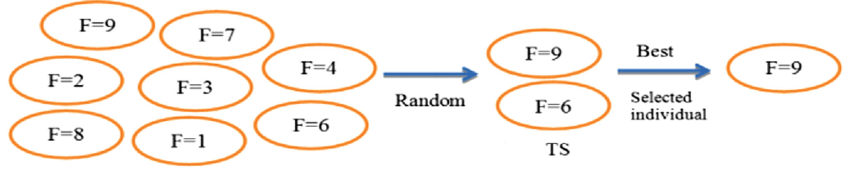
\includegraphics{img/appendixC/tournament-selection.png}
        }
        \vspace{-0.25cm}
        \caption{\tiny~Ilustración que describe el proceso de Selección de padres.~\textit{Adaptado de:}~\cite{ayoub2020}}%
        \label{fig:tournament_selection}
    \end{figure}
\end{frame}

\begin{frame}{Anexo \thesection~: Cruzamiento}%
    \vspace{-0.15cm}
    \begin{figure}[H]
        \centering
        \adjustbox{max width=\textwidth, max height=0.7\textheight}{%
            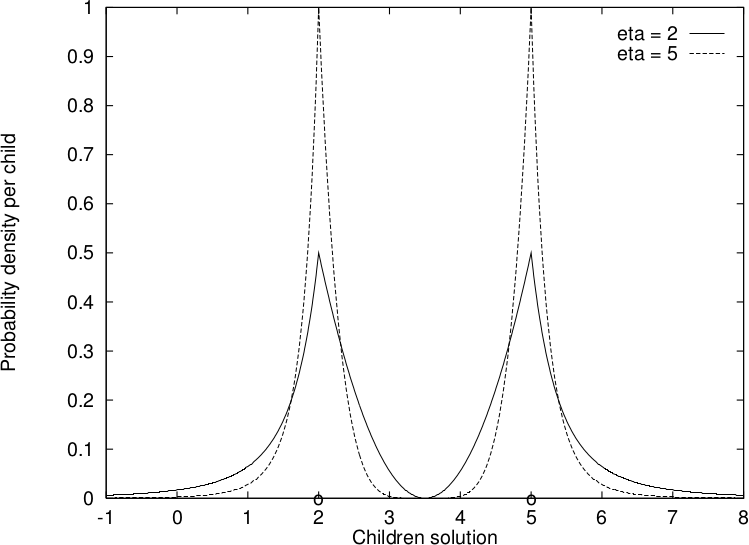
\includegraphics{img/appendixC/sbx.png}
        }
        \vspace{-0.25cm}
        \caption{\tiny~Ilustración que describe el proceso de Cruzamiento.~\textit{Adaptado de:}~\cite{stackoverflow_crossover_index_2019}}%
        \label{fig:tournament_selection}
    \end{figure}
\end{frame}

\begin{frame}{Anexo \thesection~: Mutación}%
    \vspace{-0.15cm}
    \begin{figure}[H]
        \centering
        \adjustbox{max width=\textwidth, max height=0.7\textheight}{%
            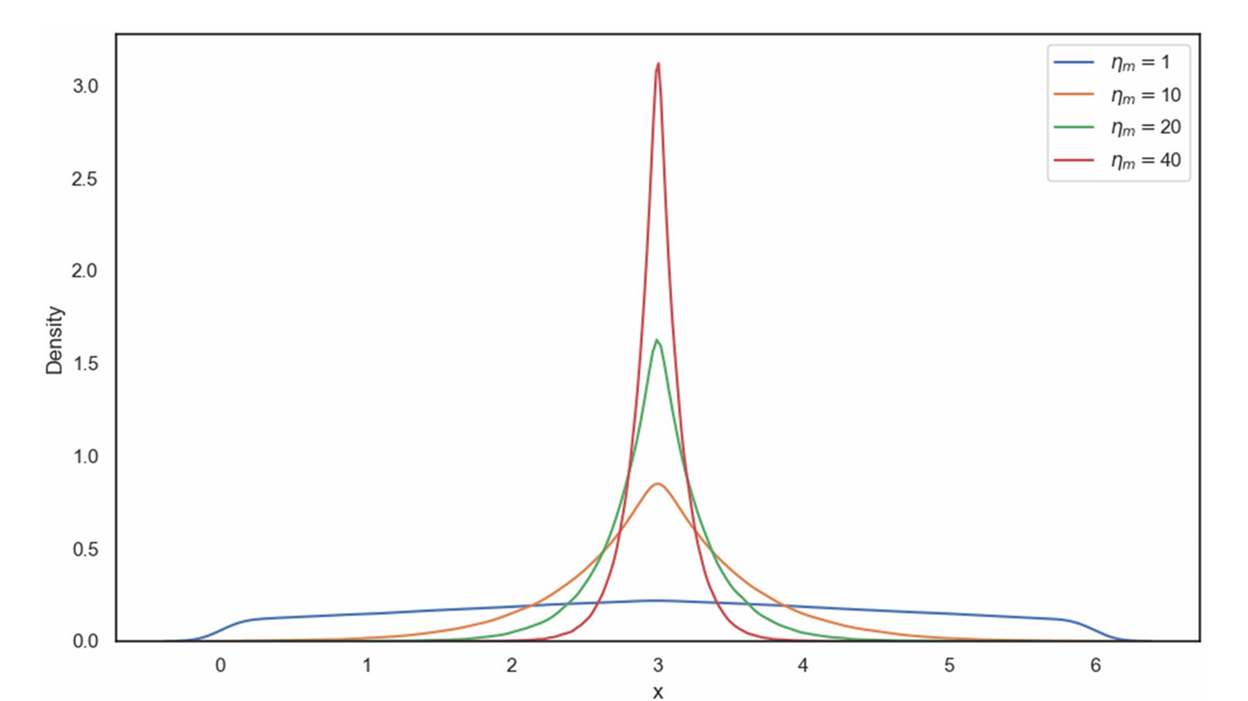
\includegraphics{img/appendixC/polynomialMutation.png}
        }
        \vspace{-0.25cm}
        \caption{\tiny~Ilustración que describe el proceso de Mutación.~\textit{Adaptado de:}~\cite{CarlesBou2023}}%
        \label{fig:tournament_selection}
    \end{figure}
\end{frame}

\end{document}